\section{Additional Experiment Detail}
\label{sec:appendix-exp}
\subsection{Large Batch Size}
To help understand where the speed-up comes from when batch size is greater than 1, we present the Union Contextual Sparsity (fraction of neurons/heads that are not used by any of the inputs in the batch) of different batches sizes for MLP and Attention blocks, respectively, in Figure~\ref{appendix:exp_sparsity_batch}. Union Contextual Sparsity is calculated as 1.0 - the union of activated MLP neurons or Attention heads in the batch / total neurons or heads. The union operation is essential to realize a fast sparse GEMM. 

Surprisingly the number of MLP neurons/Attention heads that \name{} activated does not grow linearly with the batch size. This suggests a power law distribution rather than a uniform distribution of parameter access from all input examples. Further, a larger batch size can easily lead to out-of-memory for long sequence settings due to the limited GPU memory, the giant large model size, and the stored KV cache. For example, the total GPU memory of 8 80GB A100 is 640GB. Model parameters are around 350GB for OPT175B. The KV cache for a batch size 32 with a sequence longer than 1920 tokens has already filled up the GPU memory. 

\begin{figure}[h]
  \centering
     \subfigure[MLP]{
    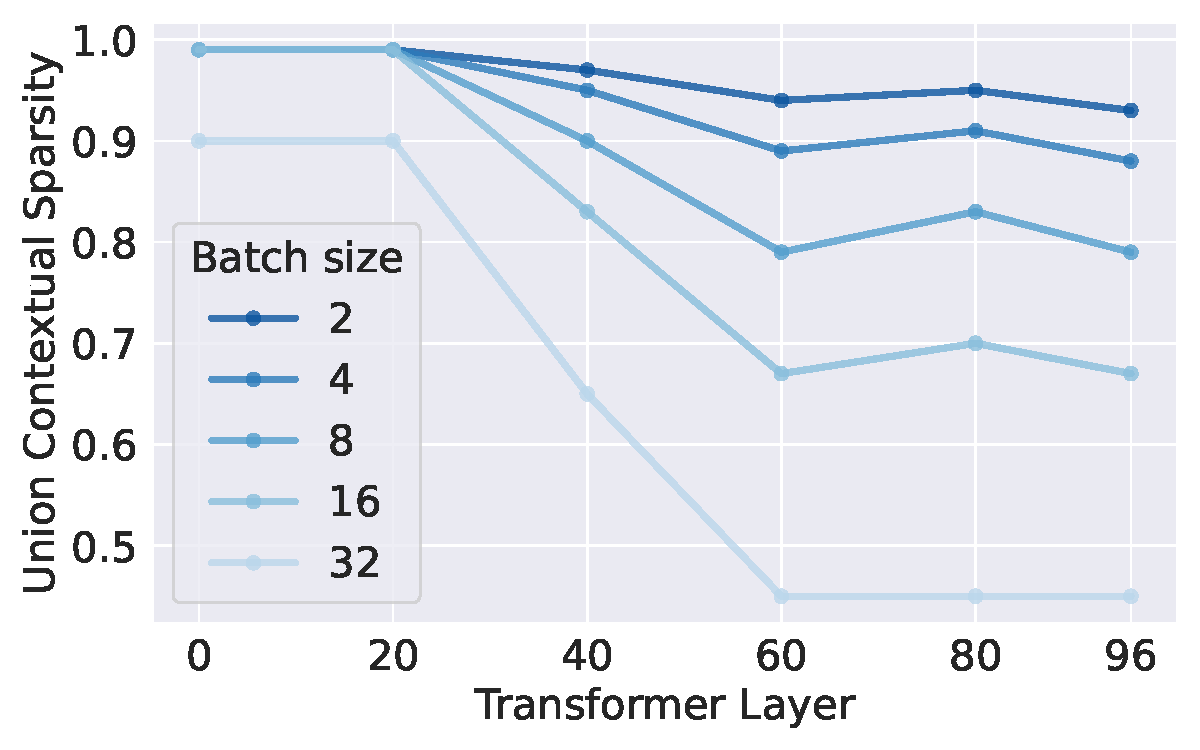
\includegraphics[width=0.40\textwidth]{figure/experiment/batch_sparsity_mlp.pdf}
    }
   \subfigure[Attention]{
    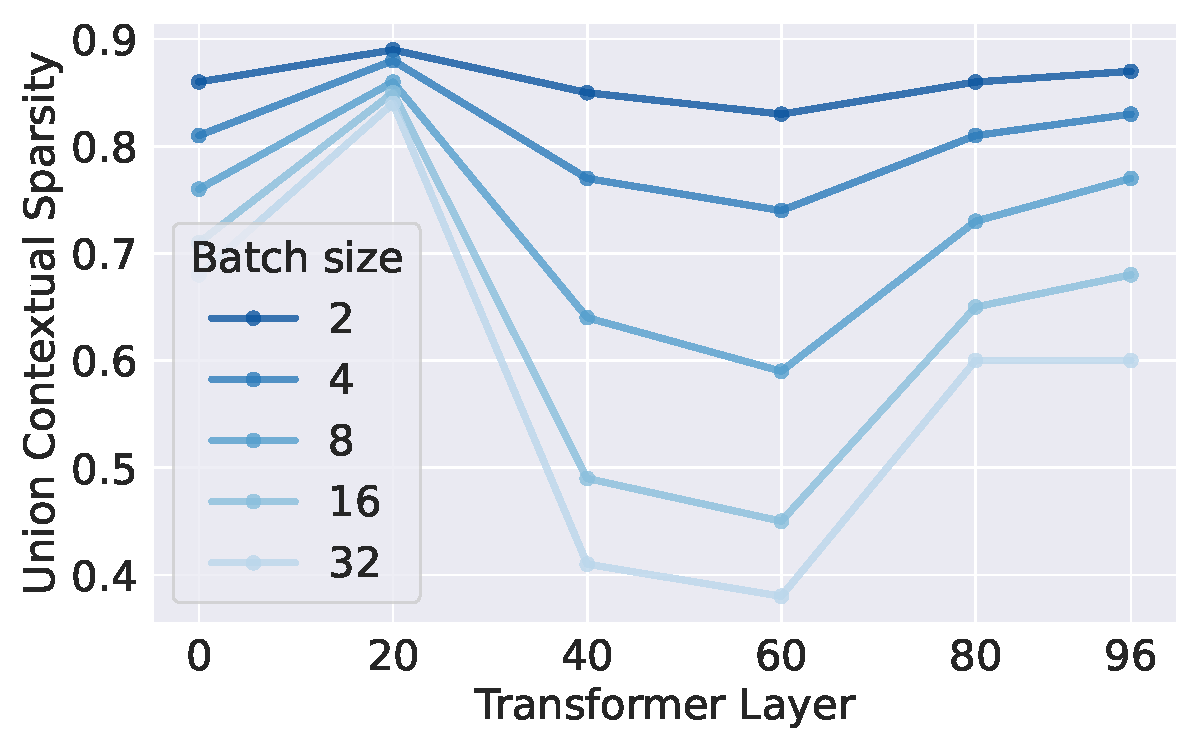
\includegraphics[width=0.40\textwidth]{figure/experiment/batch_sparsity_attention.pdf}
    }
  \caption{Union contextual sparsity with larger batch size.}
  \label{appendix:exp_sparsity_batch} 
\end{figure}
\subsection{Near Neighbor classifier}
In the \name{} framework, any near-neighbor search method under the inner product metric would be sufficient to predict a sparsity pattern. "Training predictor" is to reduce the cost of on-the-fly prediction, rather than training the model itself.

For example, in our exploration stage mentioned in Section 4.1, we adopt HNSW, a state-of-art near-neighbor search method, to predict MLP sparse pattern, and we can see from the following table there is no drop in the perplexity at 90 \% sparsity ratio. However, due to the high dimensionality of embedding and HNSW’s reliance on CPU, the time HNSW took to identify the sparsity pattern is 10ms, which is longer than the MLP computation.

\begin{table}[h]
\centering
\begin{tabular}{ccc}
\hline
          & OPT-1.3B & OPT-1.3B + HNSW \\
\hline
Hellaswag & 0.4154   & 0.4314          \\
C4        & 14.2     & 14.4           \\
\hline
\end{tabular}
\end{table}
In our paper, we choose a neural network classifier as our near neighbor search method to take advantage of the fast matrix multiplication on GPU. And training such classifiers to predict sparsity patterns is not only cheaper in terms of training cost but also inherently different from the method concept.
\subsection{Future Possibility: Skipping Layer}
\label{sec:exp_skip_layer}


\label{sec:block_parallel}
Deja Vu currently sparsifies from the perspective of model width. Here, we explore the possibility of sparsification from model depth. 
As observed in \cref{sec:obs}, we show that the activation of large language models changes slowly across blocks. This property can be leveraged to increase the efficiency of a trained model by parallelizing, reordering, or skipping certain intermediate sub-blocks without significantly impacting the overall accuracy. 
\begin{table}[t]
\scriptsize
\centering
\caption{ Sparsify from the Depth: Skipping or parallel entire transformer blocks may not lead to catastrophic drop in accuracy at test time.}
\resizebox{0.6\linewidth}{!}{
\centering
\Huge
\begingroup
\setlength{\tabcolsep}{10pt}
\renewcommand{\arraystretch}{1.3}
\begin{tabular}{l||cccccc}
\specialrule{.15em}{.05em}{.05em}
 Model & COPA & Hellaswag & Lambada & OpenBookQA & PIQA  & Winogrande	\\
\cline{1-7}
 OPT-175B        
            & 0.8600 & 0.7814  & 0.7584 & 0.4460 & 0.8096 &  0.7261 \\
 \, - Parallel 2  
            & 0.8300 & 0.7737  & 0.7762 & 0.4520 & 0.8030 & 0.7096 \\
 \, - Parallel 4  
            & 0.5200 & 0.2519  & 0      & 0.2720 & 0.5092 & 0.4870 \\
 \, - Skip 2/8  
            & 0.8000 & 0.7112  & 0.6387 & 0.4220 & 0.7840 & 0.6630 \\
 \, - Skip 2/4 
            & 0.6900 & 0.4409  & 0.0240 & 0.3400 & 0.6882 & 0.5383 \\
\cline{1-7}
Bloom         
            & 0.8000  & 0.7460  & 0.6771 & 0.4480 & 0.7949 & 0.7040  \\
\, - Parallel 2   
            & 0.8100  & 0.7404  & 0.6992 & 0.4360 & 0.7813 & 0.7048 \\
\, - Parallel 4
            & 0.6200  & 0.3176  & 0.1325 & 0.2720 & 0.5593 & 0.5217 \\
 \, - Skip 2/8  
            & 0.7900 & 0.6829  & 0.5936 & 0.4120 & 0.7699 & 0.6614 \\
 \, - Skip 2/4 
            & 0.6600 & 0.5538  & 0.3023 & 0.3580 & 0.7046 & 0.5549 \\
\specialrule{.15em}{.05em}{.05em}
\end{tabular}
\endgroup
}
\end{table}
\begin{table}[ht]
\scriptsize
\centering
\resizebox{0.3\linewidth}{!}{
\centering
\Huge
\begingroup
\setlength{\tabcolsep}{10pt}
\renewcommand{\arraystretch}{1.3}
    \begin{tabular}{lrr}
    \toprule
    Setting                 & Wiki(ppl) & C4(ppl) \\
    \midrule
    Baseline                &  11.57    &   10.17    \\
    % Parallelize  2 blocks   &           &          \\
    % Parallelize  4 blocks   &   nan     &    nan    \\
    Skip every 2 layers      &  21.16    &   16.58   \\
    Skip every 4 layers      &  13.45    &   11.37  \\
    % Skip every 8 layers      &  12.37    &           \\
    \bottomrule
    \end{tabular}
\endgroup
}
\label{table:corruption}
\end{table}


Improving the inference efficiency of Transformer models is a challenging task due to their sequential execution of Transformer layers.
Each sub-block depends on the output of the previous one, leading to low hardware efficiency, particularly during the token generation phase where each forward pass is computed for only one token.
% To address this issue, various solutions have been proposed such as pipeline parallelism \cite{} and tensor parallelism \cite{}.
However, the sequential execution of blocks and sub-blocks yields computation bubbles, and the latter involves a large amount of communication overhead. 
Here, we present an interesting observation that can potentially alleviate these challenges. We found that the activation of the model changes slowly across blocks. Specifically, the cosine similarity of activations between adjacent blocks is often above 0.99.
This suggests that the blocks might take the previous activation as input -- parallelize or reorder the blocks -- without significantly affecting the output.
Slowly changing activations suggest that it may be possible to parallelize, reorder, or even skip blocks while maintaining a similar output.
Some existing models, such as GPT-J~\citep{gpt-j}, GPT-NeoX~\citep{gpt-neox-20b}, and PaLM~\citep{chowdhery2022palm} already placed the Attention block and MLP block in parallel in training to facilitate parallel computation and reduce the communication overhead. 

Here we investigate the possibility at inference time. And surprisingly, we found parallelizing those blocks for models that are trained in a sequence manner will not hurt the performance of downstream tasks significantly. And surprisingly, we found parallelizing those blocks for models that are trained in a sequence manner will not hurt the performance of downstream tasks significantly. Table\ref{table:corruption} presents some preliminary results of OPT-175B and Bloom

Given the activation $y$ and Transformer layer $l$, we have:
\begin{align*}
    \widetilde{y}_l \leftarrow y_l + \mathsf{MHA}^{l}(y_l) \\
   \widehat{y}_l \leftarrow \widetilde{y}_l + \mathsf{MLP}^{l}(\widetilde{y}_l)
\end{align*}
Parallelizing two blocks refers to placing the Attention and MLP blocks in parallel, i.e.:
\begin{align*}
    \widehat{y}_l \leftarrow y + \mathsf{MHA}^{l}(y_l) + \mathsf{MLP}^{l}(y_l)
\end{align*}
Parallelizing four blocks then parallelize the blocks of two Transformer layers, defined as follows:
\begin{align*}
    \widehat{y}_{l+1} \leftarrow y_l + \mathsf{MHA}^{l}(y_l) + \mathsf{MLP}^{l}(y_l)
    + \mathsf{MHA}^{l+1}(y_l) + \mathsf{MLP}^{l+1}(y_l)
\end{align*}
Skipping layers is straightforward, which drops an entire Transformer layer for every $n$ layers.


We are surprised to find that parallel two layers preserve accuracy on a series of tasks across models. Besides, randomly skipping 25\% layers doesn't lead to catastrophic quality. Our findings suggest from the downstream task perspective, the activation patterns within the model are relatively consistent across different blocks, providing a potential avenue for future research on model compression and optimization.




% \begin{table}[]
%     \centering
%     \begin{tabular}{lrr}
%     \toprule
%     Setting                  & Wiki(ppl) & C4(ppl) \\
%     \midrule
%     Baseline                 &  10.82    &   8.04      \\
%     Parallelize  0.5 block   &  11.47    &   8.04      \\
%     Parallelize  2 blocks    &           &           \\
%     Parallelize  3 blocks    &   nan     &    nan    \\
%     Skip every 2 blocks      &           &           \\
%     Skip every 4 blocks      &           &           \\
% emma    Skip every 8 blocks      &           &           \\
%     \bottomrule
%     \end{tabular}
%     \caption{OPT-175B, Corruption}
%     \label{tab:opt_corruption}
% \end{table}
% \begin{table}[]
%     \centering
%     \begin{tabular}{lrr}
%     \toprule
%     Setting                 & Wiki(ppl) & C4(ppl) \\
%     \midrule
%     Baseline                &  11.57    &   10.17    \\
%     % Parallelize  2 blocks   &           &          \\
%     % Parallelize  4 blocks   &   nan     &    nan    \\
%     Skip every 2 layers      &  21.16    &   16.58   \\
%     Skip every 4 layers      &  13.45    &   11.37  \\
%     % Skip every 8 layers      &  12.37    &           \\
%     \bottomrule
%     \end{tabular}
%     \caption{Sparsify from the Depth}
%     \label{tab:bloom_corruption}
% \end{table}


% \fi



%%% Local Variables:
%%% mode: latex
%%% TeX-master: "main"
%%% End:
